\problemname{Fractal Tree}

\noindent
A fractal tree $F_i$ is defined in the following way.
First, a rooted tree $F_0$ is given, which contains at least 2 vertices.
$F_i$ is then defined recursively in the following manner.
Consider the set of vertices $S$ which are leaves in $F_{i-1}$.
For each vertex $v$ in $S$, we replace it with a copy of $F_0$, such that $v$ corresponds to the root of $F_0$.

Now, consider the tree $F_k$, for a given $k$.  In this tree, we
perform a depth-first search, where we visit all vertices of the tree
recursively.  At a certain vertex, we first recurse into the subtree
of the leftmost child of the vertex, then the second leftmost child,
and so on, until we have visited all the vertices in the subtree of
the vertex.  Assign integer labels to the vertices in the order they
were visited, starting at $1$.  See Figure~\ref{fig:fractaltree} for
an example.

\begin{figure}[h!]
    \centering
    \subfigure[The tree $F_0$.]{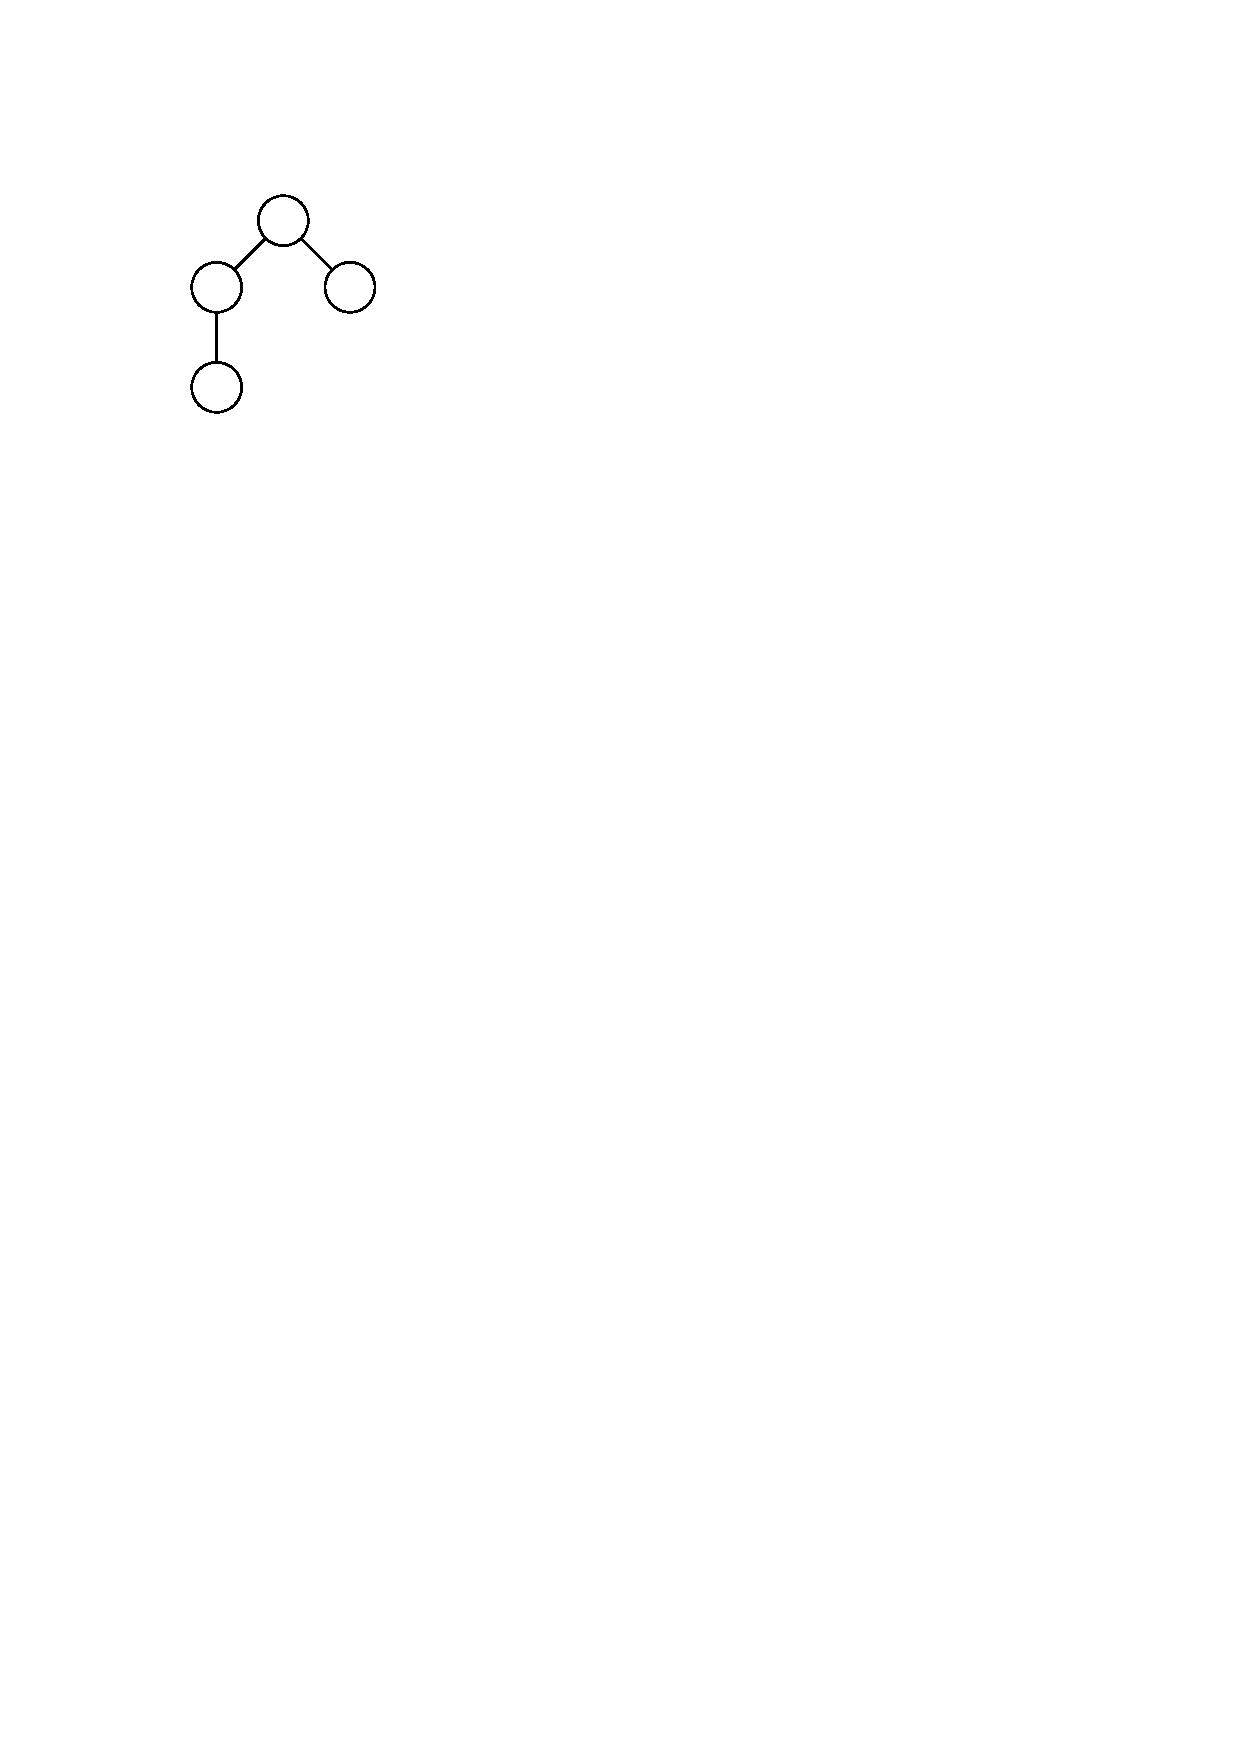
\includegraphics[width=0.24\textwidth]{sample1-f0}}
    \quad\quad
    \subfigure[The tree $F_1$.]{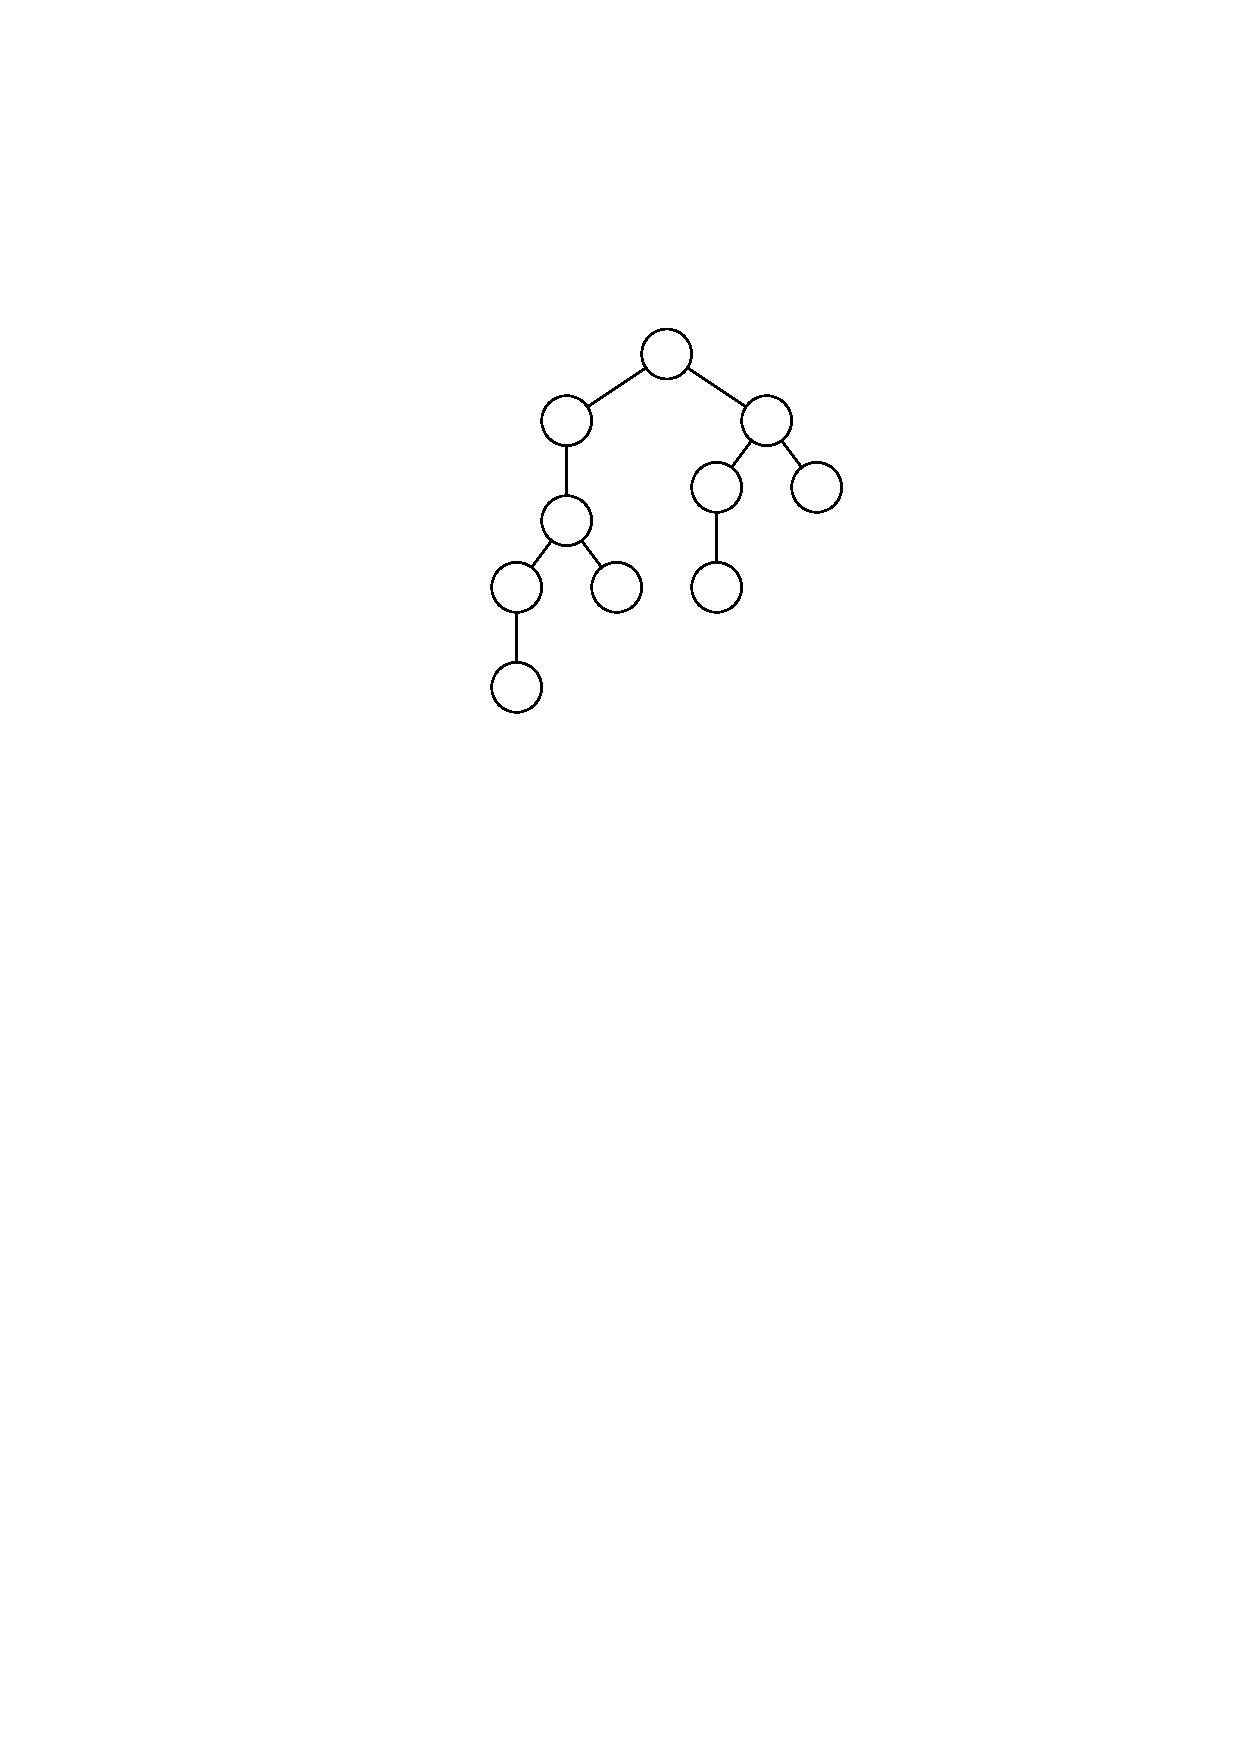
\includegraphics[width=0.24\textwidth]{sample1-f1}}
    \quad\quad
    \subfigure[The depth first search labelling of $F_1$.]{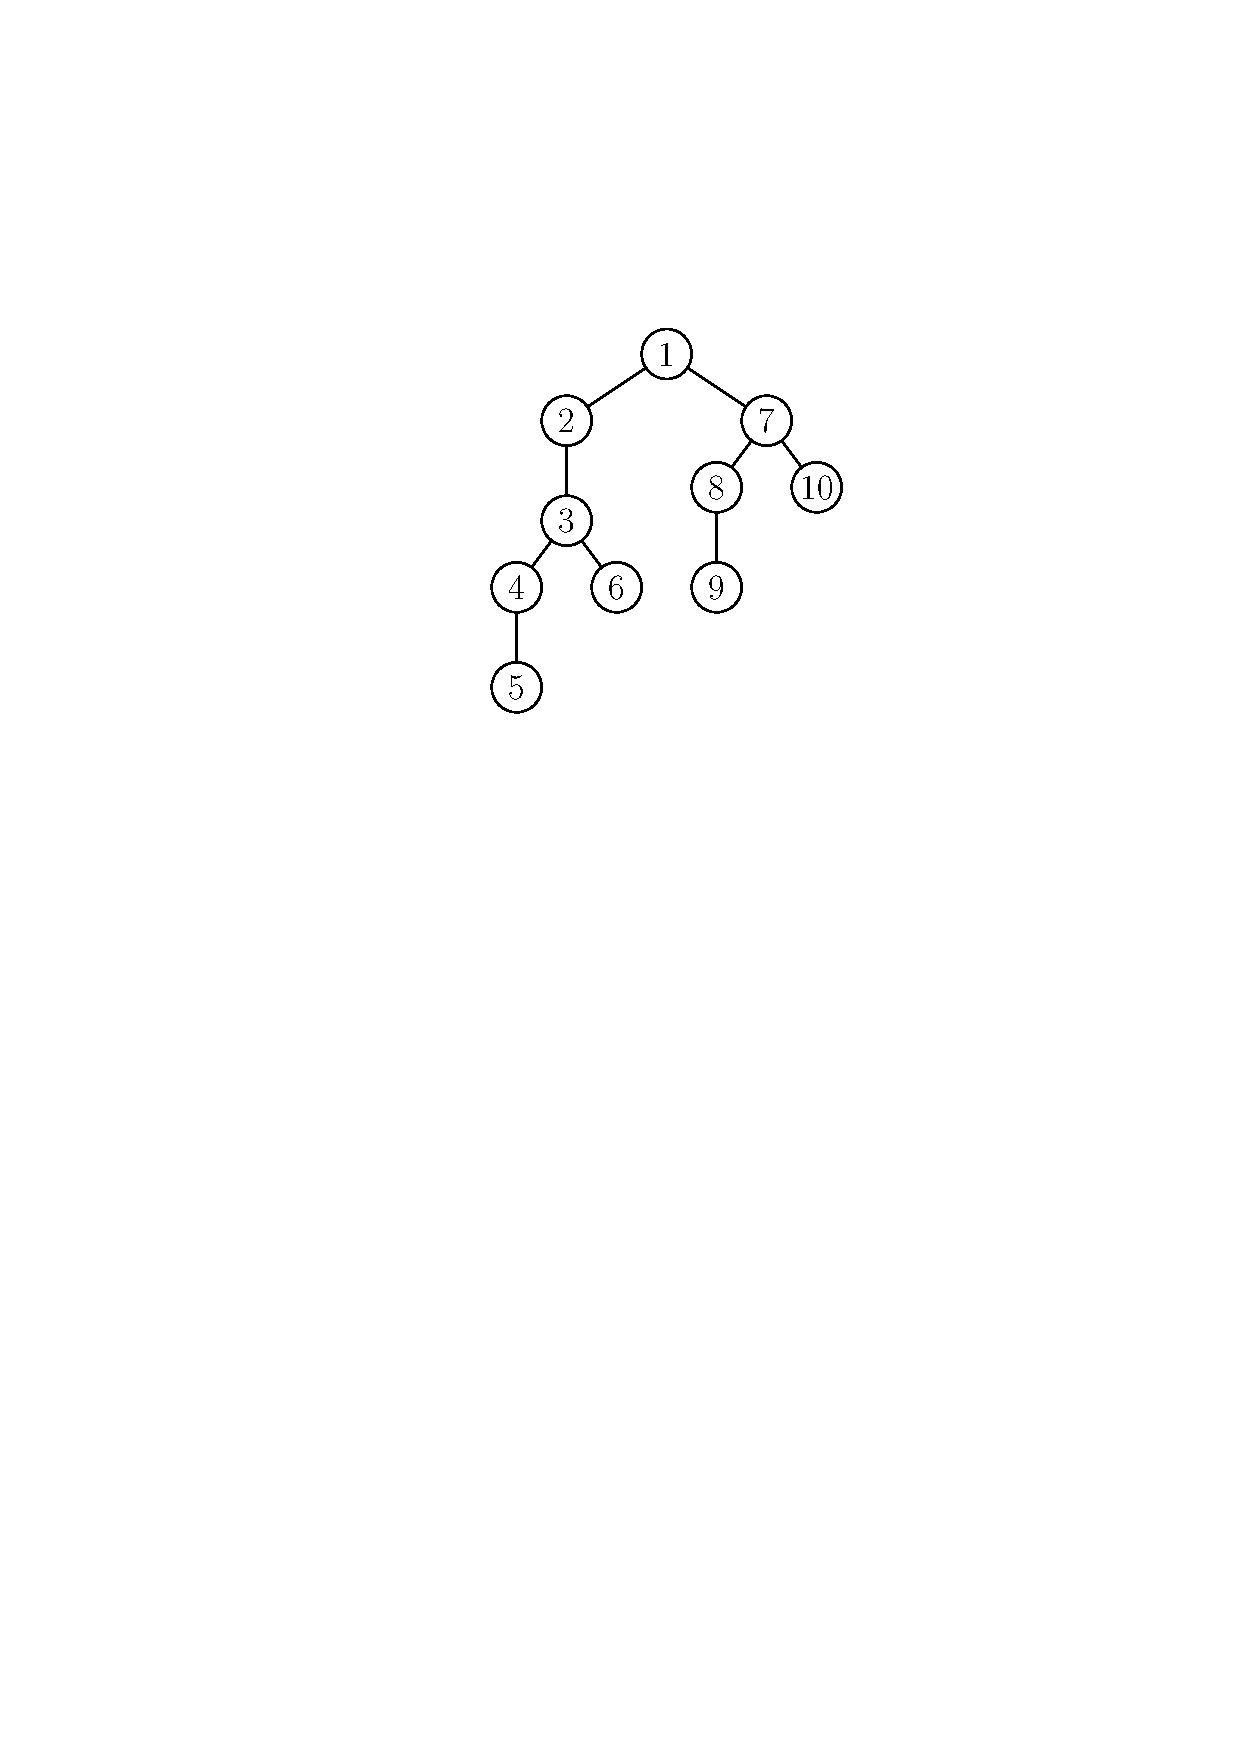
\includegraphics[width=0.24\textwidth]{sample1-f1-labelled}}
    \caption{Illustration of Sample Input 1.}
    \label{fig:fractaltree}
\end{figure}

\noindent
Given a set of queries consisting of pairs of vertices, your task is to find the distance between the two vertices.
The distance is defined as the number of edges on the (unique) simple path between the two vertices.

\section*{Input}
First, the tree $F_0$ is given.
The first line of input contains the number of vertices $2 \le n \le 100\,000$ in $F_0$.
The vertices are numbered $0$ to $n - 1$, with $0$ being the root vertex.
Then follows a line containing $n-1$ integers $p_1, \ldots, p_{n-1}$.  For each $1 \le i \le n-1$, the parent of node $i$ in $F_0$ is $p_i$.
It holds that $p_i < i$.
Within the tree, the left-to-right ordering of the vertices correspond to their numbering, in ascending order (i.e. the lowest-numbered child is the leftmost child).

The third line of input contains an integer $0 \le k < 2^{30}$.
Then follows a line containing an integer $q$, $1 \le q \le 100\,000$,
the number of queries.  Finally, there are $q$ lines containing the
queries.  Each query is given by two distinct integers $a$ and $b$, the labels
of two vertices of $F_k$.  You may assume that $a$ and $b$ are valid
labels (i.e., they are between $1$ and the number of vertices of
$F_k$), and that they are at most $2^{30}$.

\section*{Output}

For each query $(a, b)$, in the same order as given in the input, output the distance in $F_k$ between the vertices labelled $a$ and $b$.
